\section{Gramáticas incontextuales}

% \Deactivate
% $$\begin{array}{lcl}
% X_0 &\to& \lambda | 0X_0 | 1X_1\\
% X_1 &\to& 0X_2 | 1X_0\\
% X_2 &\to& 0X_1 | 1X_2\end{array}$$
% \Activate

\subsection{Gramáticas incontextuales}
\begin{easylist}[itemize]
& Una gramática incontextual (CFG de \textit{Context Free Grammar}) $G$ es un conjunto de reglas de reemplazo donde las partes izquierda son palabras de longitud 1. A las reglas también se les suele llamar \textit{producciones}.

\Deactivate
$$\begin{array}{lcl}
S &\to& aS\\
S &\to& X\\
X &\to& aXb\\
X &\to& \lambda
\end{array}$$
\Activate

& A todo símbolo que aparezca a la izquierda de alguna regla lo llamaremos \textit{variable} o \textit{no terminal}. Generalmente, los denotamos con letras mayúsculas.

& Al resto de símbolos los llamamos \textit{terminales} y, normalmente, los notamos con letras minúsculas.

& En este caso, $S$ y $X$ son variables mientras que $a$ y $b$ son terminales.

& Usualmente la lista de reglas se representa de forma comprimida agrupando las partes derecha de regla de cada variable. Por ejemplo: 

\Deactivate
$$\begin{array}{lcl}
S &\to& aS\; | \; X\\
X &\to& aXb \; | \; \lambda
\end{array}$$
\Activate

& En una gramática, siempre se distingue una variable inicial, llamada \textit{símbolo inicial} (en este caso, $S$) que, por defecto, es la primera que aparece.

& Las palabras generadas por la gramática son las formadas por terminales y que sean alcanzables desde el símbolo inicial.

& Ejemplo de derivación de $G$: vamos reemplazando los símbolos subrayados por los resultados de las reglas de reemplazo. Así: $\underline{S} \to_G a\underline{S} \to_G a\underline{X} \to_G aa\underline{X}b \to_G aab$. Esta palabra ya es terminal. Así pues, $aab$ es una palabra generable por la gramática $G$.

& Una derivación se puede representar, también, en forma de árbol. En la raíz situamos el símbolo inicial. Vamos colgando en cada sustitución los cambios que hacemos.

\ \begin{tikzpicture}[level distance = 10mm, sibling distance = 10mm]
\node {$S$}
child {node {$a$}}
child {
    node {$S$}
    child {
        node {$X$}
        child {node{$a$}}
        child {
                node{$X$}
                child {node{$\lambda$}}
            }
        child {node{$b$}}
    }
};
\end{tikzpicture}

& La palabra generada será la concatenación de todas las hojas: $aa\lambda b = aab$. A este tipo de árbol se le llama \textit{árbol sintáctico}.

& A veces, las CFG se representan más formalmente con una tupla $G = \langle V, \Sigma, \delta, S\rangle$ que contiene el alfabeto de variables o no terminales, el alfabeto de  símbolos no terminales, el conjunto de reglas y cuál de las variables es el símbolo inicial.

& En el ejemplo anterior, $$G = \langle \{S, X\}, \{a, b\}, \{S \to aS, S\to X, X \to aXb, X\to\lambda\}, S\rangle.$$

& El lenguaje generado por una gramática se define como el conjunto de palabras formadas por símbolos terminales y generables desde el símbolo inicial: $\mathcal L (G) = \{w\in \Sigma^* \colon S\to_G^* w\}$.

& El lenguaje generado por una variable concreta de la gramática es el conjunto de palabras terminales generables desde esa variable: $\mathcal L(G, X) = \{w \in \Sigma^* \colon X\to_G ^* w\}$.

& El ejemplo anterior genera el lenguaje $\mathcal L(G) = \{a^nb^m\ \colon n \geq m\}$. Esto es, las palabras con unas cuantas $a$s seguidas de unas cuantas $b$s donde hay más o igual $a$s que $b$s.

& A un lenguaje se le llama lenguaje incontextual, o CFL si existe una gramática que lo genera: $L \in \textrm{CFL} \iff\exists G \in \textrm{CFG} \colon \mathcal L(G) = L$.

& Existen algoritmos para comprobar si una palabra es generable por una gramática y, en caso afirmativo, construye un árbol de generación o sintáctico.

& El árbol es útil pues nos estructura una palabra de entrada que, inicialmente, no era más que una secuencia de símbolos. Por ejemplo, relación entre lenguajes de programación y compiladores.

& Una gramática alternativa equivalente a la anterior es $S \to aS \;|\; aSb \;|\; \lambda$. En este caso, hay un solo no terminal. Desde $S$ podemos escoger si añadimos una $a$ o añadimos una $a$ y una $b$ al mismo tiempo.

& Esta gramática tiene un problema: tiene árboles de derivación diferentes para una misma palabra $aab$.

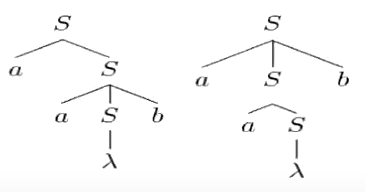
\includegraphics{t4-2.png}

& Cuando una gramática permite más de un árbol de derivación para alguna palabra, decimos que es \textit{ambigua}.

& Otra gramática ambigua es:

\Deactivate
$$\begin{array}{lcl}
E &\to& E + E \; | \; E - E \; | \; N\\
N &\to& ND \; | \; D\\
D &\to& 0|1|2|3|4|5|6|7|8|9
\end{array}$$
\Activate

& Una expresión puede ser suma de expresiones o resta de subexpresiones o un número. Un número puede ser uno o más dígitos.

& Podemos generar la palabra $7 - 4 + 2$. \textit{A priori}, la palabra no significa nada.

& Hay dos árboles de derivación diferentes para esta palabra.

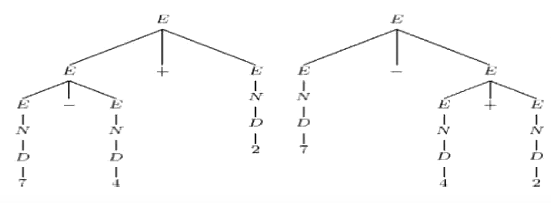
\includegraphics{t4-3.png}

& Ambos árboles son útiles para comprobar que nuestra palabra de entrada pertenece a la gramática. Sin embargo, los árboles de derivación se pueden usar luego para dar significado a las palabras que generan.

& En el caso de la izquierda, resulta que primero hay que restar $7$ y $4$ y luego la suma de $2$ y la subexpresión anterior. En el otro, es al revés.

& En el supuesto caso que usemos un generador automático de árboles sintácticos a partir de una gramática y una entrada, si la gramática es ambigua, corremos el riesgo de que los árboles obtenidos no se correspondan a la interpretación que queremos dar a las entradas. Por ese motivo, el motivo de ambigüedad es importante y conviene tenerlo en cuenta al usar reconocedores automáticos.

& Una gramática equivalente a la anterior y no ambigua es
\Deactivate
$$\begin{array}{lcl}
E &\to& N + E \; | \; N - E \; | \; N\\
N &\to& ND \; | \; D\\
D &\to& 0|1|2|3|4|5|6|7|8|9
\end{array}$$
\Activate

& Nótese que estamos obligados a escoger la primera regla si el primer operador es suma, y la segunda regla si el primer operador es resta. De este modo, la palabra que queremos generar determina de forma unívoca la regla a utilizar en cada nodo.

\end{easylist}








\subsection{Operaciones sobre gramáticas incontextuales}
Cuando operamos dos lenguajes incontextuales con ciertas operaciones conocidas, el resultado es, nuevamente, un lenguaje incontextual.


\subsubsection{Unión}

\begin{easylist}[itemize]
& Los lenguajes incontextuales son cerrados por unión: si hay gramáticas para $L_1$ y $L_2$, entonces $L_1, L_2 \in \textrm{CFL} \implies L_1 \cup L_2 \in \textrm{CFL}$.

& Sean $G_1 = \langle V_1, \Sigma_1, \delta_1, S_1\rangle$ y $G_2 = \langle V_2, \Sigma_2, \delta_2, S_2\rangle$ gramáticas tales que reconocen los lenguajes $L_1$ y $L_2$; esto es, $\mathcal L(G_1) = L_1$ y $\mathcal L(G_2) = L_2$.\footnote{También hemos de suponer que $V_1 \cap V_2 = \varnothing$. Esto es, que no comparten variables libres. Pero esto no conlleva una pérdida de generalidad, pues, sin ningún problema podemos renombrar las variables en una de las gramáticas de manera que aquella gramática siga generando el mismo lenguaje.}

& La unión de $L_1$ y $L_2$ es, y notado abusivamente, $L_1 \cup L_2 = \langle V_1 \cup V_2 \cup \{S\}, \Sigma_1 \cup \Sigma_2, \delta_1 \cup \delta_2 \cup \{S \to S_1 | S_2\}, S \rangle$.

& Esto es, añadimos una nueva regla a partir de $S$: $S_1$ o $S_2$.

& Por tanto, $\mathcal L(G_1 \cup G_2) = \mathcal L(G_1) \cup \mathcal(G_2) = L_1 \cup L_2$.
\end{easylist}


\subsubsection{Intersección}
\begin{easylist}[itemize]
& Los lenguajes \textit{no} están cerrados por interseccción: esto es, que $L_1, L_2 \in \textrm{CFL}$ no implica $ L_1 \cap L_2 \in \textrm{CFL}$.

& Por ejemplo, no es difícil encontrar gramáticas para los lenguajes $\{a^nb^nc^m \colon n,m \geq 0\}$ y $\{a^nb^mc^m \colon n,m\}$ (ambos $\in \textrm{CFL}$); pero su lenguaje intersección, $\{a^nb^nc^n \colon n \geq 0\}$ no es incontextual, como veremos en otra sección.

\end{easylist}

\subsubsection{Complementario}

\begin{easylist}[itemize]
& Los lenguajes tampoco están cerrados por complementario. Si lo estuviesen, como $L_1 \cap L_2 = \overline{\overline{L_1} \cup \overline{L_2}}$, entonces la intersección también sería una operación cerrada para lenguajes incontextuales, cosa que hemos visto que no es así.
\end{easylist}


\subsubsection{Concatenación}

\begin{easylist}[itemize]
& Los lenguajes incontextuales están cerrados por concatenación: $L_1, L_2 \in \textrm{CFL} \implies L_1 \cdot L_2 \in \textrm{CFL}$.

& Esto es, sean $G_1 = \langle V_1, \Sigma_1, \delta_1, S_1\rangle$ y $G_2 = \langle V_2, \Sigma_2, \delta_2, S_2\rangle$ gramáticas tales que reconocen los lenguajes $L_1$ y $L_2$; esto es, $\mathcal(G_1) = L_1$ y $\mathcal (G_2) = L_2$, con $V_1 \cap V_2 = \varnothing$.

& $G_1 \cdot G_2 = \langle V_1 \cup V_2 \cup \{S\}, \Sigma_1 \cup \Sigma_2, \delta_1 \cup \delta_2 \cup \{S \to S_1S_2\}, S \rangle$. La diferencia está en que, ahora, desde el símbolo inicial de la gramática generamos la concatenación de $S_1$ con $S_2$.

& De esta manera, desde $S$ podemos generar todas las palabras que se forman al concatenar una palabra de $L_1$ con otra de $L_2$.

& Así pues, queda claro que generamos el lenguaje concatenación de $L_1$ y $L_2$: $\mathcal L(G_1 \cdot G_2) = \mathcal L(G_1) \cdot \mathcal L(G_2) = L_1 \cdot L_2$.
\end{easylist}

\subsubsection{Estrella}
\begin{easylist}[itemize]
& Los lenguajes incontextuales están cerrados por la operación estrella. Es decir: si $L \in \textrm{CFL}$, entonces $L^* \in \textrm{CFL}$.

& Si $G = \langle V, \Sigma, \delta, S\rangle$ tal que $\mathcal L(G) = L$, entonces $G^* = \langle V \cup \{S'\}, \Sigma, \delta \cup \{S' \to S'S|\lambda\}, S'\}$ cumple $\mathcal L(G^*) = \mathcal L (G)^* = L ^*$.

& Añadimos una regla tal que, desde $S'$, generamos $0$ o más $S'$s; esto es, $0$ o más palabras de $S$.
\end{easylist}

\subsubsection{Reverso}
\begin{easylist}[itemize]
& Los lenguajes incontextuales están cerrados por reverso. Es decir: si $L \in \textrm{CFL}$, entonces $L^R \in \textrm{CFL}$.

& La gramática reverso se obtiene simplemente manteniendo las mismas reglas pero haciendo el reverso de sus partes derecha.

& $G^R = \langle V, \Sigma, \{X \to u^R \colon (X \to u) \in \delta\}, S'\rangle$. Esto es, $\mathcal L(G^R) = \mathcal L(G)^R = L^R$.\footnote{Mirad \url{https://youtu.be/rHOyFDCOKbs} a partir del minuto 5:26 para una justificación exhaustiva de esta propiedad.}
\end{easylist}







\subsection{Depuración de gramáticas (1)}
\begin{easylist}[itemize]
\end{easylist}

\textit{Falta redactarlo}





\subsection{Depuración de gramáticas (2)}
\begin{easylist}[itemize]
\end{easylist}


\textit{Falta redactarlo}




\subsection{Depuración de gramáticas (3)}
\begin{easylist}[itemize]
\end{easylist}

\textit{Falta redactarlo}